\documentclass[12pt]{article}
	\usepackage[T1]{fontenc}
	\usepackage[utf8]{inputenc}
	\usepackage[british]{babel}
	\usepackage[a4paper]{geometry}
	\geometry{verbose,tmargin=3cm,bmargin=3cm,lmargin=2cm,rmargin=2cm,marginparwidth=70pt}
	\setcounter{secnumdepth}{3}
	\setcounter{tocdepth}{3}
	\setlength{\parindent}{4em}
	\setlength{\parskip}{1em}
	\renewcommand{\baselinestretch}{1.5}
	\usepackage{prettyref}
	\usepackage{textcomp}
	\usepackage{booktabs}
	\usepackage{lscape}
	\usepackage{setspace}
	\usepackage{indentfirst}
	\usepackage{fancyhdr}
	\usepackage{url}
	\usepackage[normalem]{ulem}
	\usepackage[table, fixpdftex]{xcolor}
	\usepackage{algpseudocode}
	\usepackage{bigstrut}
	\usepackage{enumitem}
	\usepackage{verbatim}
	\usepackage{mathtools}
	\usepackage{graphicx}
	\usepackage{longtable}
	\usepackage{chngpage}
	\usepackage{pdfpages}
	\usepackage[all]{nowidow}
	% package hyperref
    \usepackage[hidelinks]{hyperref}
  

	% biblatex
	\usepackage[style=authoryear,natbib=true,maxcitenames=2, maxbibnames=11,backend=biber,pagetracker=page,hyperref=true]{biblatex} \usepackage{csquotes}
	\renewcommand*{\bibsetup}{%
		\interlinepenalty=10000\relax % default is 5000
		\widowpenalty=10000\relax
		\clubpenalty=10000\relax
		\raggedbottom
		\frenchspacing
        \biburlsetup}
        
	% fixes the page number of the first page of each chapter
	\fancypagestyle{plain}{
			\fancyhead{}
			\renewcommand{\headrulewidth}{0pt}
			\renewcommand{\footrulewidth}{0pt}
			\fancyfoot[OC]{\begin{flushright}\thepage\end{flushright}}
    }
    
	% fancy headers for the thesis
	\fancyhead{}
	\fancyhead[RO]{\slshape \nouppercase \rightmark}
	\fancyfoot[OC]{\begin{flushright}\thepage\end{flushright}}
	\renewcommand{\headrulewidth}{0.4pt}
	\setlength{\headheight}{14pt}

	% add bibliography database
	\addbibresource{BA copy.bib}
	
	% space between biblio items
	\setlength\bibitemsep{1.7\itemsep} 
	
	% title without ""
	\DeclareFieldFormat[inbook]{title}{#1}
	% non-italic
	\DeclareFieldFormat[online]{tlaitle}{#1} 
	% title unquoted
	\DeclareFieldFormat[article]{title}{#1} 
	% no pp. 
	\DeclareFieldFormat[article]{pages}{#1} 
	% bold volume
	\DeclareFieldFormat*{volume}{\mkbibbold{#1}\setpunctfont{\textbf}}
	
	% no in:
	\renewbibmacro{in:}{} 
	
	% (volume)
	\renewbibmacro*{volume+number+eid}{%
			\printfield{volume}%
			%\setunit*{\adddot}% DELETED
			% \setunit*{\addnbspace}% NEW (optional); there's also \addnbthinspace
			\printfield{number}%
			% \setunit{\addcomma\space}%
			\printfield{eid}}
	\DeclareFieldFormat[article]{number}{\mkbibparens{#1}} 
	
	% edition.
	\DeclareFieldFormat{edition}%
	{(\ifinteger{#1}%
			{\mkbibordedition{#1}\addthinspace{}ed.}%
			{#1\isdot}).}
	
	% publisher and location p osition
	\renewbibmacro*{publisher+location+date}{%
			\printlist{publisher}%
			\setunit*{\addcomma\space}%
			\printlist{location}%
			\setunit*{\addcomma\space}%
			\usebibmacro{date}%
			\newunit}
	
	% shortauthor before author
	\renewbibmacro*{begentry}{%
			\ifkeyword{Key}{\sffamily}{}%
			\iffieldundef{shorthand}
			{}
			{\global\undef\bbx@lasthash
					\printfield{shorthand}%
					\addcolon\space}%
			\ifboolexpr{test {\usebibmacro{bbx:dashcheck}} or test {\ifnameundef{shortauthor}}}%
			{}%
			{\printnames{shortauthor}%
                    \addspace\textendash\space}}
                    
\title{The Importance of the Investing Corporation's Financial Condition in the Presence of Schedule 13(D) Filings}
\author{Leopold Ingenohl}


\begin{document}
\maketitle

\pagebreak


\section{Introduction}

\begin{center}
	Macht das überhaupt Sinn was ich schreibe? Kann man das nachvollziehen? 
\end{center}
% rethink sentence - not reporting requirements! 
Much attention has been recently given to the current Securities and Exchange Commission (SEC) reporting requirements for Schedule 13(D), governing the disclosure of beneficial ownership interests in excess of five percent of outstanding common stock of a U.S. public company \citep{Giglia2018}. Amongst other causes, it is due to significant gains for the subject's stock when a partial acquisition through a Schedule 13(D) filing is announced \citep{Akhigbe2007}. 

% types of filer - bridge corporations
However, it is still largely unanswered where this upward drift comes from \citep{Greenwood2009}. An approach to this issue is objective of this thesis. Namely, analyzing the link between the financial condition of corporate investors and the abnormal returns on the subject's stock and determining whether the financial condition has explanatory power for the latter. The following findings motivate this approach.  


In recent studies of what happens to the target's stock after such a filing, \citet{Collin-Dufresne2015} observe a positive significant market reaction to the subject's stock upon a more general sample of Schedule 13D filings 
	\footnote{The sample is only restricted on the subjects stock characteristics rather than on characteristics of the filers e.g. they exclude all filings which are not common stock (CRSP share code 10 or 11), whose prices are below \$1 and above \$1000 and which involve derivatives \citep{Collin-Dufresne2015}.}. 
\citet{Brav2008} have shown a favorable market reaction, 7\% - 8\% average abnormal returns in the (-20|20) event window, particularly to Schedule 13D's filed by hedge funds. Similar results have been shown by \citet{Klein2009} who observe 10.2\% average abnormal stock returns specifically for hedge fund targets.\\
In addition, \citet{Brigida2012} have shown an even higher runup if the acquirer is a private investor or a non-financial corporation. This is matching with \citet{Akhigbe2007} findings who observe greater gains for the target's stock if the partial position was initiated by a corporate bidder. Concluding, filings submitted by all investor types are followed by positive market reactions on the subject's stock but those submitted by corporations seem to have a stronger impact. This motivates the first hypothesis which assumes significant positive abnormal returns for Schedule 13(D)'s filed by corporations.
% Characteristics | Motivation | Reasoning - Why do they make minority acquisitions? 

Since the investing corporation is allowed to behave in an activist manner by filing a Schedule 13(D) 
	\footnote{In comparison the investor could file a Schedule 13(G) in which he would hold the shares passively hence with no intention to bring change.} 
\citep{Brigida2012} they can use their stakes to actively monitor and influence the target which is similar to the definition of an entrepreneurial activist by \footnote{\citet{Klein2009} define the entrepreneurial activist as an investor who buys a large stake in a publicly held corporation with the intention to bring change and thereby realize a profit on the investment.} \citet{Klein2009}.
These stakes tend to be either made for the purpose of investment or far more importantly, as strategic investments \citep{Damodaran2005}, possibly resulting in business agreements, alliances or joint ventures \citep{Allen2000}. \\
% Topics: Acquisitions | Friendly Takeovers | Hostile Takeovers | Joint-Venture | Activism | Comparison | Comparison HF - Why do they behave activist? 
In a more direct approach however, these strategic investments can also help as a stepping stone towards full control \citep{Huang2017}. 
This approach is supported by \citet{Goldman2005} who find that mergers and takeovers are often preceded by the acquisition of a minority stake in the target. Whereas hedge funds use their stakes to change characteristics of the target (e.g. the board of directors or the strategic orientation) \citep{Klein2009} corporate filers are mainly focused on synergies in the form of strategic alliances or takeovers between them and the target. \citet{Akhigbe2007} observe that partial acquisitions, if carried out by corporate investors, are more likely to result in a full acquisition when compared to all other activist investors. This means that within the mass of Schedule 13D filings, institutional investors are unlikely to pursue a complete takeover whereas corporations are potential full acquirers \citep{Brigida2012}. The possibility of a takeover could be one explanation for the strong impact corporate filings have on the market, because the abnormal returns could be a reflection of investors' expectations of the target firms stock being acquired at a premium to the current price \citep{Goldman2005} especially with strong corporate bidders being likely to overpay in the event of a full takeover \citep{Akhigbe2007}.
These findings motivate the second hypotheses which assumes the highest abnormal returns occur in the event of a purpose of transaction statement involving a merger or a takeover of the subject.
%Objective: highlight the importance of the financial condition -- Background

However, in order to be able to bring change -- might it be in the form of a strategic alliance or eventually in a takeover -- the filing corporation should be in a condition of sufficient financial health. 
% insert the method of payments in a takeover 
A recent example on this matter is the public perception of the HNA Group. The financial condition of the HNA group, China's largest private conglomerate which over the past few years invested around \$US40 billion in businesses around the world, has currently been of great interest to financial news. Not least because they built up a 9.9\% stake of of around \$US4 billion in Deutsche Bank in 2017, which is just below the 10\% threshold above which stake purchases must be approved by Germany's financial watchdog but also because of their complex and nontransparent financing methods.
The financing of the group has come under strain as a result of an official crackdown on risky financing at acquisitive private enterprises in China. The highly leveraged group is now facing a potential cash-shortfall and liquidity issues resulting in a S\&P global rating downgrade referring to a a „deteriorating liquidity profile" of HNA. Although HNA group is a private conglomerate, the financial condition of corporations seems to be of great importance to other market participants with that said, even in the context of minority acquisitions. Therefore, linking investors' financial condition to  underlying market reactions could be an explanation for the latter. This motivates the third and most important hypotheses, namely that abnormal returns, triggered by activist minority acquisitions, can be explained by the financial condition of the investor. 
% payment method in takeovers! 

% Topics: Abnormal Returns | Financial Condition | Activism | Hypothesis | Conclusion

Based on the previous findings of corporate activism, namely their strong impact on the subjects stock in the form of abnormal returns and future possibilities involving the target, the economic significance of corporations as filers of Schedule 13(D)'s seems to be apparent.

Yet in order to make these possible developments and expectations look credible -- amongst other things strategic alliances and takeovers -- the investing corporation somehow has to emit signs of sufficient financial strength. Therefore, the link between the financial condition of the investor and the subsequent abnormal returns on the target's stock is an interesting issue to examine. This in particular, is objective of the paper. What precisely are the effects of Schedule 13(D) filings by corporations on the subject's stock and can the financial condition of the corporation explain the market's reaction? Or in other words -- how important is the financial condition of the corporation behaving in an activist manner? 

The paper proceeds as follows. In the Section 2, the relevant literature is being reviewed. Section 3 describes the data and sample composition. In Section 4 the market's response to Schedule 13(D) filings are being examined. Section 5 represents the ............
by  are being described.  In the section 4, being described 


\begin{comment}
	\section{Hypotheses}

\begin{enumerate}
	\item There are significant positive abnormal returns after the Schedule 13(D) filing of a corporation
	\item The purpose of the transaction has an effect on the market reaction 
	\item The financial condition of the investor can explain the market reaction
	\item The financial condition is most important, when the puspose of transaction invovles a future merger or takeover
	\item The financial condition looses its importance when the target is a poorly performing company and gains importance when the target is performing well 
	\item 
\end{enumerate}
\end{comment}


\section{Literature Review}

\subsection{Schedule 13(D) Filings}
%Topics: Historical Background | Information contained | Difference G and D
Section 13(d) of the Exchange Act of 1934 was passed in order to increase regulation of tender offers and accumulations of stock and the "growing use of cash tender offers as a means for achieving corporate takeovers."  
It acts as an early warning, signaling "every large, rapid aggregation or accumulation of securities, regardless of technique employed, which might represent a potential shift in corporate control" (FAQ). 
This means that under Section 13(d), anyone who becomes the beneficial owner of 5\% of an issuer's equity securities registered under Section 12 of the Exchange Act must file with the SEC a Schedule 13(D) within 10 days after the acquisition. The filing informs investors about individuals who could influence or change control of the issuing company \citep{Giglia2018}. Whereas filing a Schedule 13(D) allows the investor to behave in an active manner, a passive investor can file a Schedule 13(G) instead of a Schedule 13(D). It is a short-form filing that can be utilized if an investor holds a beneficial ownership interest passively, with no intent to change control of the company \citep{Giglia2018}. Within the Schedule 13(D) filings is information important to the following analysis. They specify (1) the security and the issuer, subject to the filing, (2) the identity and background of the filer, (3) the source and amount of funds or other conssiderations and most importantly, (4) the purpose of the transaction. Concluding, a Schedule 13(D) filing contains all information relevant in order to assess the underlying acquisition of at least 5\% of outstanding stock. The filers can be broadly classified into institutional investors (e.g. hedge funds, mututal funds), other entrepreneurial activists (e.g. individuals) \citep{Klein2009} and corporations. 

\subsection{Hedge Fund Activism}
%Topics: Characteristics AR | Problems in Comparison | Motivation of HF | Activism
There have been many studies that examined the effect a Schedule 13(D) filing submitted by hedge funds has on the target firm's stock price. In the presence of short-hprizon event studies of stock returns they all find positive abnormal returns for the subjects stock around the filing date. 
\citet[p.1730]{Brav2008} find positive average abnormal returns in the range of "7\% to 8\% during the (-20,+20) announcement window for activist hedge funds. \citet{Klein2009} have similar findings and observe 10.2\% average abnormal stock returns for hedge fund targets. In contrast, \citet{Greenwood2009} observe average abnormal announcement returns of 2.36\% for a sample of activist portfolio investors and document that the ability to force the target into a takeover is the driving force behind the abnormal market reaction. In a more recent study by \citet{Denes2017}, they average the valuation effect to around 5\% on the target's stock if submitted by hedge funds. It can be seen that all studies observe positive abnormal returns around the filing date but differ in their magnitude (Comparing the the returns can be misleading as the authors used different models for computing the abnormal returns)
	\footnote{\citet{Greenwood2009} use the market return model with matching portfolios and the CAR for aggregated abnormal returns; \citet{Brav2008} calculates the aggregated abnormal returns by subtracting the value-weighted market index from the buy-and-hold return; \citet{Klein2009} use a similar approach with buy-and-hold returns but make more adjustments.}.
Although the filing of a Schedule 13(D) can be seen as the trigger for the market reaction, the reason of why the abnormal returns occur is still largely unknown. However, \citet{Brav2008} find that if hedge funds engage actively, they have a high succession rate in achieving their main objectives. In a more recent paper conducted by \citet[p.12]{Brav2009} they list these objectives based on the sample of filings. The vast majority of these objectives focuses on general characteristics of the target and possible increase in shareholder value. They can be separated into five, not mutually exclusive, categories. The first objective is the believe of the hedge fund that he can help the manager maximize the shareholder value because they believe that the company is undervalued. The second includes activism that is based on the targeting firm's payout policy and capital structure. for the third objective, the hedge funds target issues related to business strategy, such as operational efficiency, mergers and acquisitions or growth strategies. The fourth objective is aimed at the sale of the target company with the majority to force a sale of the target company to a third party. The last objective includes activism targeting corporate governance. These motives are congruent with the \citet{Klein2009} definition of an entrepreneurial activist "who buys a large stake in a publicly held corporation with the intention to bring about change and thereby realize a profit on the investment". A more cautious definition is presented by \citet{Greenwood2009} who define an activist investor as someone who tries to change the status quo through voice, without a change in control of the firm. While all of these studies involve a deepened investigation of hedge-funds, especially their impact and motivation, most of them leave the remaining investor types aside.

\subsection{Minority Acquisitions}
%Topics: General Objectives | Definitions | Motivation | Minority Acquisitions | Toehold 

While the objectives of hedge funds in the light of Schedule 13(D) filings  have been discussed in many studies, there is still much more debate on the motivation of corporations to engage in such minority acquisitions. 
Corporate investments in other firms' equities can be be split in two broad categories. They can either be classified as ordinary investments or far more importantly as strategic investments. For the latter they could serve as a first step to engage with the opposing company. This is assumption is verified by \citet{Allen2000}, \citet{Ouimet2013} and \citet{Huang2017} who find that corporations make minority acquisitions in other companies when they confront informational or integration barriers -- in one way or another, they want to engage with the target.

The decreasing barriers give rise to business agreements, alliances, joint ventures or takeovers. In the sense of possibilities that might be reached, corporate ownership, in comparison to ownership by institutional investors, is unique
	\footnote{In \citet{Allen2000} sample, the mean fraction of equity acquired in the sample is 20\% with blockholdings of at least 5\% of voting shares. This is similar in size to the underlying sample of the paper.}
\citep{Allen2000}.
%Business agreements 
If a business agreement demands one party to invest in an asset and the value of the asset is determined by future trade between the parties, the investing party might be concerned with a holdup problem of the partner 
	\footnote{\citet{Ouimet2013}Defines the holdup problem as a decrease in it's bargaining power in a renegotiation of the contract  because the value of the initial investment is dependent on future trade with the partner.}.   
To encourage and hedge the investment and to further ensure collaboration, the investor can buy a minority stake 
	\footnote{\citet{Ouimet2013} defines acquisitions as minority acquisitions if less than 50\% have been acquired, majority acquisitions otherwise.}
in the partner \citep{Ouimet2013}. The minority acquisition can help to mitigate incomplete contracts and thereby facilitate cooperation between the two partners \citep{Allen2000}. 
Another form of cooperation induced by a minority acquisition is the direct financing of the target by the acquirer. As noted by \citet{Ouimet2013}, the investment helps to overcome asymmetric information helping to certify the target for other outside investors.
In a more strategic approach, undertaking a minority acquisition is of help to better assess real options, notably that of expanding. The acquisition of a minority stake helps to better assess the target for a potential majority acquisition \citep{Ouimet2013} and to gather more information before launching a bid for a takeover \citep{Huang2017} - minority acquisitions can help as a stepping stone towards full control \citep{Huang2017}.

Because there are two options two acquire a publicly traded firm in the United States, either through a merger or through a tender offer \citep{Offenberg2015}, \citet[p.1]{Mitchell2011} use the term takeover "for any acquisition of corporate control through the purchase of the voting stock of the target firm, regardless of whether the bid is in the form of a merger agreement or a tender offer". Whereas a merger agreement is the result of negotiations between the investor and the target's management, in a tender offer the acquirer makes a direct bid to target shareholders to purchase the target shares.
By negotiating with the target's management a merger agreement might appear as the safer option. However, it does not lock up the target from potential competition because the director fiduciary duties require the target board to evaluate competing offers until the agreement is approved by the shareholders \citep{Mitchell2011}. In the case of a merger agreement, the beneficial ownership of a partial stake can thus help to speed up the shareholder approvement process, induce the acquirer to fully commit to the merger and therefore increases the probability of a successful takeover. To prohibit the acquirer of purchasing target shares in the market during negotiations, parties often sign a standstill agreement \citep{Mitchell2011}. In contrast, shareholders of the target might sign a voting agreement in favor of the acquirer in which they agree to vote the shares in a way expressed by the acquirer - corporations might have to sign a Schedule 13(D) although they did not buy the shares but have their voting power. 

Another possibility is the purchase of ownership in the target prior to the start of the takeover bid - a toehold. Neither management nor target's shareholders know of the acquirers takeover intention. Following \citet[p.158]{Eckbo2009} acquiring a toehold, before initiating the takeover bid, is compelling. It reduces the number of shares that must be bought at the full takeover premium and it can be sold at a profit if a rival bidder winds the target but it can also create hostility with the target's management \citep{Goldman2005}. This is the reason why toeholds are much more common in hostile bids \citep{Mitchell2011}. On the other hand \citet[p. 216]{Povel2014} suggest that toeholds are not much different to the general minority acquisitions. Because the toeholder might negotiate the right to nominate one or more directors in the target's board, they open the door to a more intensive cooperation. According to \citep{Mitchell2011} bidders initiating a takeover bid in the U.S. over the period 1980-2005 offered all cash as payment in 26\% of the cases, all stock in 37\%, and a mix of both in 37\%.

Concluding, corporations filing a Schedule 13(D) and confessing their intent to behave in an active manner have many motives to do so. However, overcoming informational and integration barriers seems to pervade in almost all cases. Nevertheless, a strong engaging investor is a representation of the investment's future stability and value creation and stands for further possible engagements with the target. 

Considering the takeover process mentioned above, the necessity to file a Schedule 13(D) and thereby confirm the beneficial ownership of at least 5\% of the outstanding stock, prior or while negotiating the takeover bid, is more difficult to comprehend. Nevertheless the success of a potential takeover seems to be especially dependent on the bidders condition to be faster and stronger than potential competitors, the initial bidder has to ensure assertiveness. In order to appear strong (the market perceives the acquirer as a winner) the acquiring company must have sufficient financial strength. In the first place to make the takeover process credible to outside investors and secondly to signal the ability to pay the takeover premium. In any case, the target's outstanding shares have to be acquired at a premium to the price prevailing at the filing date either trough cash, stock or a mix of both. Besides that, a strong acquirer could have more bargaining power in persuading the target's shareholders to approve the merger and successfully carry out the takeover. 

\section{Data}

\subsection{Constructing the Sample}
% Why Schedule 13(D)filings - Klein 
The data used to conduct the following analysis is primarily composed of information gathered from Schedule 13(D) filings 
	\footnote{Schedule 13(D) filings are "the mandatory federal securitites law filings under Section 13(d) of the 1934 Exchange Act that investors must file with the SEC within 10 days of acquiring more than 5\% of any class of securities of a publicly traded company if they have an interest in influencing the management of the company" \citep[p. 1736]{Brav2008}} 
within SEC's Edgar database and further from data provided by Wharton Research Data Services (WRDS). The sample of Schedule 13(D) filings is conctructed as follows. First, using an automatic search script, 48'626 filings from the 20 year period starting in January 1996 and ending in December 2016 were identified.  The script identifies all Schedule 13(D) filings that appear on EDGAR and extracts the following information: name of filer and subject, the CUSIP of the underlying security and the filing date. Next, to only have filings submitted by corporations hence to separate corporate investors from institutional investors (i.e. hedge-funds, pension-funds or real estate investment trusts (REITs), 10-K reports were cross-referenced with the initial sample of all filings
	\footnote{10-K reports were used to identify corporations because "managers of publicly traded firms are required to produce public documents that provide a comprehensive review of the firm’s business operations and financial condition and an important financial disclosure document created by managers to communicate with investors and analysts is the annual report filed pursuant to the Securities Exchange Act of 1934 the Form 10-K." \citep[p. 1643]{Loughran2014}}. 
In order to be part of the sample, the filer had to have a 10-K report submitted 12 months prior to the filing which reduced the sample to 3'325 filings. Because the daily stock returns and prices for the underlying securities come from the Center for Research in Security Prices (CRSP) the subject not only had to have SEC's CUSIP identifier but also an active link between its CUSIP and CRSP's unique PERMNO identifier. For the remaining 1'467 filings, there had to be sufficient data on CRSP in order to calculate the abnormal returns for the subjects which reduced the sample to 1'151 filings. 
The accounting fundamentals, needed to compute the filers financial condition, come from the COMPUSTAT database which means that the filer has to have a link between its 10K-CIK and COMPUSTAT's unique GVKEY indentifier. After crossreferencing with the remaining 1'151 filings, the sample was reduced to 1'014 filings. In the next step, according to Fama \& French's industry classification code, all filers belonging to the trading industry (Code 47) were dropped which left a sample size of 898 filings. In a last step, size and purpose of the transaction were manually extracted from the Schedule 13(D) filings, while in the process Schedule 13(D/A) filings (e.g. amendments to previous filings) that were mistakenly classified as original Schedule 13(D) filings and filings not submitted by corporations were excluded 
	\footnote{The only exception were filings submitted by the Commerce Group Inc., which provides both insurance and, real estate, brokerage services. These filings were excluded because (1) the largest part of them were amendments, (2) the amount of filings submitted was disproportionately and (3) all purposes of the transaction were as general investments in a fund.}.
which reduced the sample to 748 filings. 

\subsection{Descriptive Data}
Table 1 describes the general composition of the sample's Schedule 13(D) filings. In column (1) the complete sample of firms is being described, whereas column (2) and (3) present information on sub-samples of filings submitted by either strong or weak investors, respectively
	\footnote{The separation of firms into strong and weak ones is based on Piotroski's F-Score. Strong firms are within a score of (7-9) whereas weak firms have scores between (0-3) which is in accordance with \citet[p.12]{Mohr2012}}.
Panel A gives general characteristics of the sample's Schedule 13(D) filings. The total sample consists of 498 filings submitted by firms with 110 submitted by strong and 85 by weak. That is a difference of around 5\% with regards to the total sample but can be considered as unsubstantial with regards to the analysis. 
Following, the filings were submitted by 394 different investors but reported only 394 different subjects. This means that occasionally either one firm was investing in multiple targets (e.g. 6 filings submitted by AT\&T) or a target was subject to more than one filing (e.g. four filings in which Clearwire Inc. is target). However, in comparison to the total sample size, these pattern do not occur frequently.\\
In the ten-year span from 2002--2011, over 60\% of the total number of filings were submitted. The peak of filings was in the 5-year span before the financial crisis. It is noticeable that the number of filings in the period around the financial crisis is higher than the number of filings in the following five years. An explanation could be the merger wave of 2007 \citep[p.19]{Huang2017} increasing the need to file Schedule 13(D)'s. Strikingly, a total of 30\% of these filings were submitted by strong firms and only 12\% by weak firms, indicating that potentially a large part of the mergers were carried out by strong firms.
	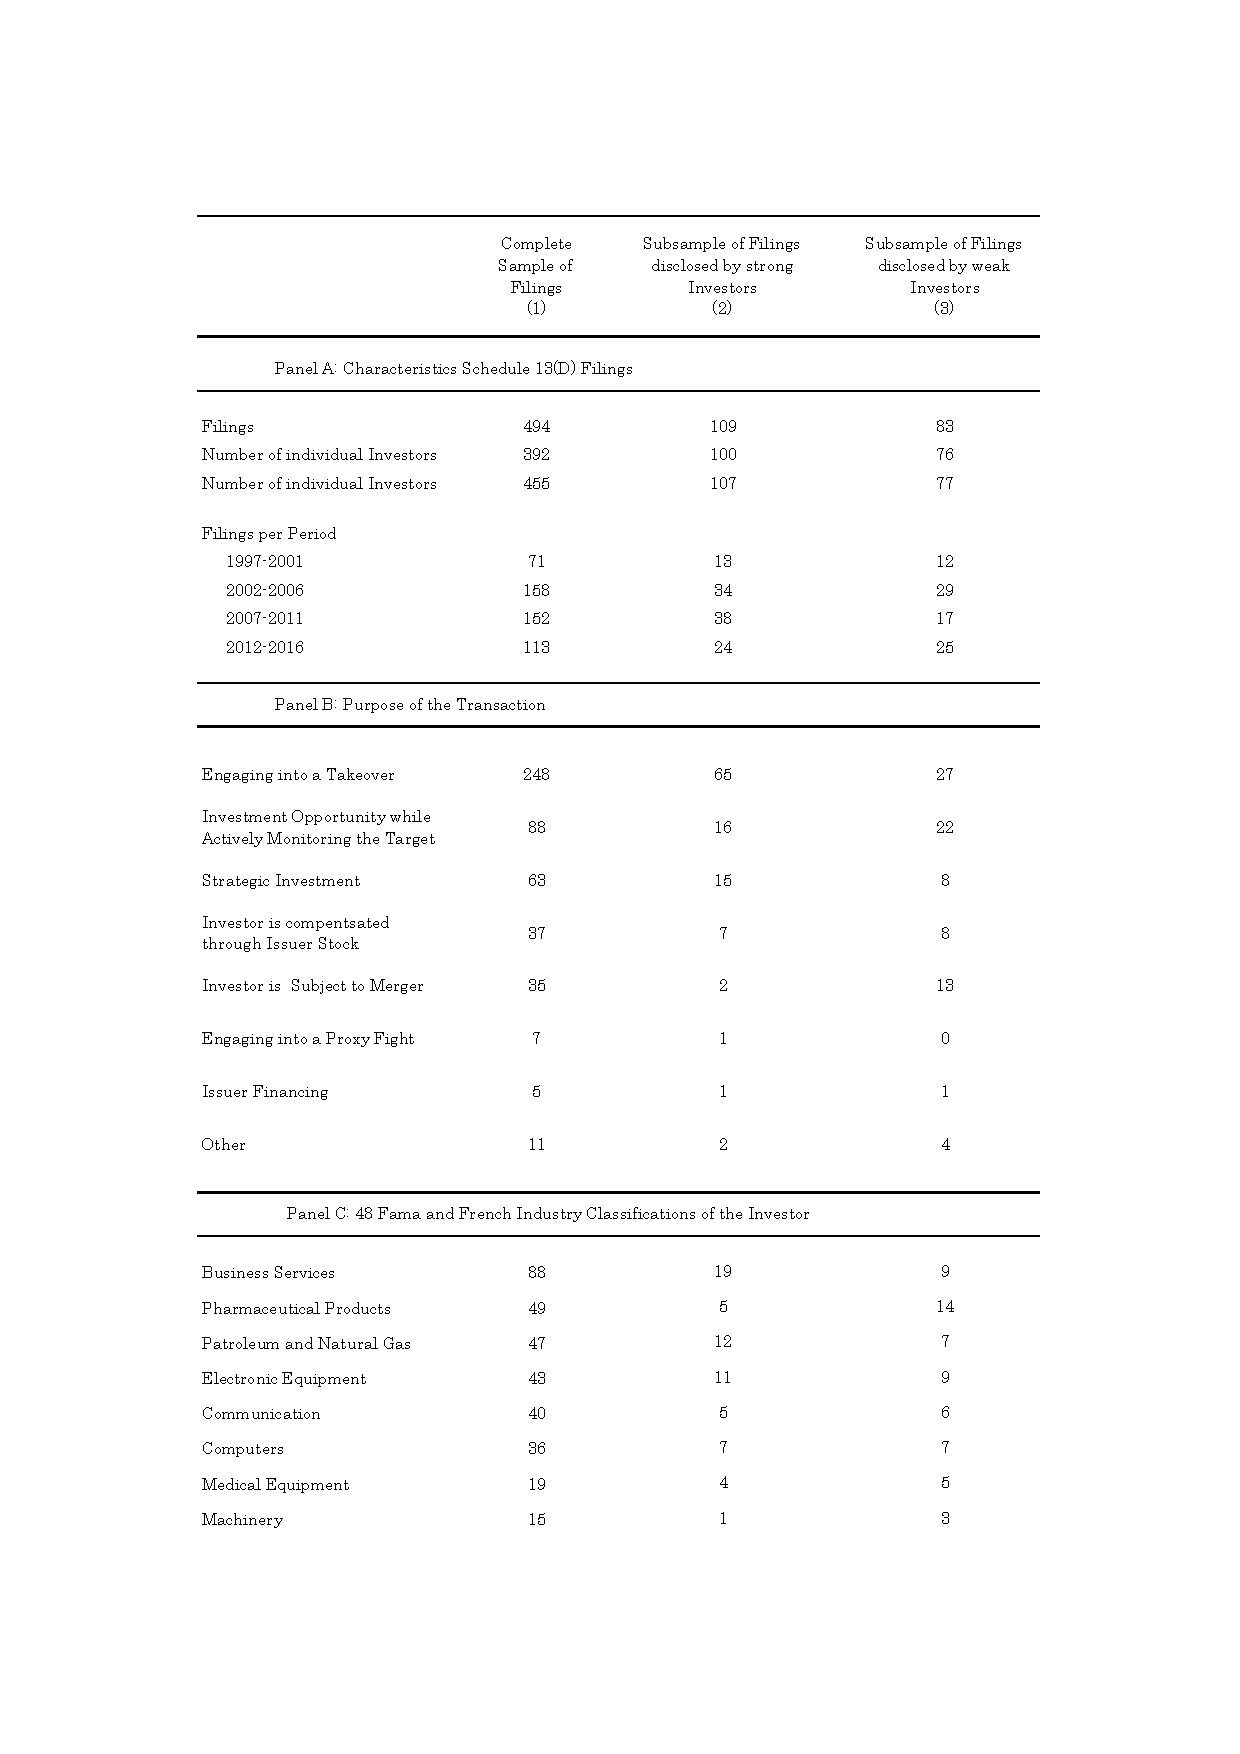
\includepdf[pages={1},pagecommand={}, width=\textwidth]{Descriptive_Statistics_copy.pdf}
Panel B lists the "Purpose of Transaction" which represents item 4 of a Schedule 13(D) filing. For simplicity and larger sub-samples, these purposes have been grouped into the following six categories. The reporting person (1) is engaging in a takeover process and, vice versa (2) became the target of a takeover, (3) actively and (4) strategically invests into the target firm, (5) is being compensated and lastly (6) reports other purposes. Detailed information on how the filings were categorized can be found in Appendix A.

The category of engaging into a takeover process, controls for all filings stating either a merger agreement, a tender offer or a hostile bid with merger agreements being the most frequently reported purposes and hostile bids the least.
Remarkable is the fact that around half of the stock acquisitions were made in the course of engaging into a takeover process. This information is important in two ways: It implies firstly that the timing component plays an important role in analyzing the market reaction around the filing date and secondly that for around half of the sample the financial condition already plays an important role. Correspondingly, more than double the amount of "takeover filings" were submitted by strong firms when compared to weak firms.\\
On the other hand, the ratio is switched for filings in which the firm acquires the stock in the course of becoming the target. This can be understood in the way that the target's shares were acquired in order to compensate own shareholders at the event of acquisition. Now, 37\% of the filings were submitted by weak firms compared to only 6\% by strong firms.\\
The second most reported purpose for firms to acquire the stock was to actively monitor the investment. Table II reports 86 of those filings. This kind of investment is based on several assumptions, which include the believe that the target's stock is undervalued (a simple investment opportunity) or the possibility to get a first glimpse at the firm. However, the bottom line is that these investments do not directly imply a value creating interaction between the two parties for the future.\\
Following actively held investments, strategic investments were made in 55 of the filings. Different to the former, they are based on the premise of future collaboration between investor and target. A strategic investment represents amongst others the realization of an alliance agreement, a license agreements or that of a joint venture. Although potentially very interesting for the coming analysis, they represent only 10\% of the filings.\\
Eventually the filings are also submitted because the "acquiring" firm is being compensated for pending payments in the form of the target's stock. This supports \citet{Ouimet2013} concept that minority acquisitions can be carried out in order to help financing the target.

Panel C is a representation of the investing firms industries according to the (48) Fama \& French industry classification code with the three-digit SIC code in brackets. In the total sample, 42 out of the maximum 48 industries are represented in the sample. Panel C only shows industries that represent at least 15 investing firms. As mentioned in Section X, the sample is restricted by excluding the trading industry due the irregular investment behavior of the corresponding firms. The two highest industry representations with more than 50 firms are computer software and pharmaceutical products. Interestingly, they have switched representations of strong and weak firms with 16 (7) and 5 (15) firms. The top two industries for strong firms were computer software and petroleum and natural gas and for weak firms pharmaceutical products and electronic equipment. 
\begin{comment}
	\subsection{Examples of Corporate Activism}
	In this subsection, two cases of corporate investments into other firms are being described. The first example is takeover the second is strategic investment. 

	\subsubsection{Pfizer Inc. and Icagen Inc. }
	On June 24, 2011 Pfizer filed a Schedule 13(D) in which it declared an ownership of 14.2\% in Icagen Inc.. Pfizer was initially engaging with Icagen in accordance to a "collaboration agreement" dated August 13, 2007. In the purpose statement of June 24, 2011 Pfizer wrote: 
	\begin{center}
		"Pfizer is evaluating the possibility of entering into a strategic transaction with Icagen, which could have the effect of influencing or changing the control of Icagen by means of stock or asset acquisition or merger"
	\end{center}
	Consequently, the filing can be considered as firms strategic investment and the purpose statement can be classified as indicating that Pfizer wants to further strategically invest in Icagen.
	The ownership of 14.2\% in Icagen was acquired between 2007 and 2008. The collaboration agreement on August 13, 2007 involved the "discovery, development, manufacture \& commercialization of pharmaceutical compounds and products that modulate three specific sodium ion channels as potential new treatments for pain and related disorders". The investment resulted in Pfizer appointing the treasurer and president of Icagen as their proxies. 
	In order to extend the collaboration agreement, on September 17 2009 Pfizer and Icagen entered into the first amendment to the agreement. 
	On September 21, 2010, one year later, they entered into a second amendment to the collaboration agreement which would extend it until December 31, 2011. In the course of a further collaboration between Pfizer and Icagen after the expiration of the collaboration agreement , Pfizer filed this Schedule as stated in the purpose statement above.
	\pagebreak	
\end{comment}

\section{Properties of Investing Firms prior to the Schedule 13(D) Filings}

% Objective: How can we identify the investor and what are the financial characteristics? 
% Topics: Strength Measurements | Why these Measures - Hypotheses |  Information in Table II |  General Financials | Comparison Targets |

% Introduction - why ? 
After being familiar with general characteristics of the sample's filings, this section focuses on identifying the investors with regards to their financial condition. The section proceeds as follows. It starts by introducing the two indicators and scores used to separate the investors into sub-samples given their indicator and score value. The section proceeds by identifying the financial characteristics for both, the total and the four sub-samples. This is done to contextualize the tools for testing the main hypothesis, namely that the investing firm's financial condition is important to the market reaction. The measurements are also established in order to enrich the explanatory power of ratio analysis.
In order to do that, the financial condition has to be broken down into quantifiable components that represent the general characteristics of profitability, liquidity, solvency and operational performance. Piotroski's F-Score is used as a measurement of general firm strength, Altman's Z-Score represents a measurement of bankruptcy and both the Whited-Wu- and KZ-Index identify financially constrained firms. A detailed explanation on the composition and calculation of the measurements can be found in Appendix 

% Information contained in Table II | Why Control Sample?
% Table II presents a summary of these indicators. Column (1) and (2) show the figures of the firms from the sample and the control sample, respectively. In order to show how the sample firms compare to their respective control samples, their means (medians) are shown side-by-side. The control sample is based on industry and size and is established to put the sample of investors into perspective and further characterize them through a direct comparison.  Column (3) presents the significance levels for tests for difference between sample and control firm's means and medians. For all tests, the $t$-statistics are for difference in means, assuming unequal variances between the samples. The $Z$-statistic is a Mann-Whitney rank-sum test of unmatched pairs. \footnote{All measurements are winsorized at the 1\% and 99\% levels so that extreme values are replaced by the respective percentiles. This enables a presentation of more meaningful mean statistics \citep{Klein2009}.}. 

% Strength Measurements
% Topics per Measure: What is it | Special Characteristics | Why is it used 
For example, in a study of 2010 \emph{BCG} notes many of that year's acquisitions would involve a financially strong acquirer. But because the attribute of being financially strong can be difficult to isolate, Piotroski's F-score is used as proxy in this sense. This is done for the two reason that it generally addresses the issue as a "... composite measure of firm strength" \citep[p. 496]{Fama2006} and considers in what directions the fundamentals of a company are trending and whether general health conditions are met \citep[p.5]{Mohr2012}. Although \citet{Piotroski2000} established it to separate strong from weak value firms
	\footnote{In order to legitimize the explanatory power of the F-score in separating strong from weak firms Piotroski formed portfolios consisting of value firms. In doing so, he showed that an investment strategy of shorting expected losers (weak firms) and buying expected winners (strong firms) would "generate a 23\% average annual return" \citep[p. 4]{Piotroski2000}. This is matching with \citet{Hyde2014} results, who observe significant return premiums for stocks with a high F-score over stocks with a low F-score.}
\citet{Mohr2012} shows that its application on growth stocks yields similar results
	\footnote{This is in line with \citet{Piotroski2000} and confirms earlier research conducted by him.}.
And even though the score was developed to distinguish among firms based on their stock performance, its application on the sample of investors will yield results that support a general understanding of financially weak and strong firms. The score consists of nine binary signals that form a final score between zero and nine, with a score of zero signaling a firm is in bad condition and a score of nine the firm is in a state of financial strength. 
Although a firm might be in the lower region of the score, it does not imply that it can be automatically called weak. For simplicity and consistency however,investors within the range of (0-3) points are labeled as weak investors and firms with a score between (7-9) are labeled as strong investors. These limits are different to Piotroski's original application but they yield larger sub-samples which are more independent from rare outliers \citep[p.12]{Mohr2012}.

With the Whited-Wu- and the KZ-Index two measures of financial constraints complement the overall picture of the investor's financial condition. Based on their indicator's value, each separates the sample in financially constrained and unconstrained firms. This is done on the following grounds. Under the assumption of perfect capital markets, the financial structure of the investor should be irrelevant to investment because "external funds provide a perfect substitute for internal capital" \citep[p. 141]{Fazzari2016}. This however, is not the case for financially constrained firms because they face an inelastic supply of external capital \citep[p.1]{Farre-mensa2013}. Consequently, firms who are able to raise substantial amounts of external capital without much of an increase in the cost of capital are considered as unconstrained \citep[p.1]{Farre-mensa2013}. If a firm is constrained, likewise faces a significant cost disadvantage of external finance, then the investment is driven by fluctuations in the cash flow \citep[p. 142]{Fazzari1988}. This means that in the presence of asymmetric information, the internally generated cash flow is the most likely source of funds for corporate investments \citep[p.450]{Bhagat2005}. Consequently, the firm invests less when it faces a decrease in internal funds \citep[p.451]{Bhagat2005}, also known as investment-cash flow sensitivity. Amongst others, this is why both indices include the dividend payouts in their formulas, as firms paying out dividends are more independent on cash-flow fluctuations hence can be classified as financially unconstrained.
The KZ-Index is based on a logit model relating the degree of financial constraints to five accounting variables: cash flow, market value, debt, dividends and cash holdings, each scaled by assets \citep[p.5]{Farre-mensa2013}. Although \citet{Khatami2014} notes that more recent literature has questioned the reliability of constraint measures, the Whited-Wu- and KZ-Index as defined in \citet{Farre-mensa2013} are used as indicators for the latter. For both indices firms are sorted into terciles based on their index values. Firms in the top tercile are coded as constrained those in the bottom tercile are coded as unconstrained. This results in 166 constrained and 166 unconstrained firms.


To further enrich the measures, Altman's Z-score is included. The Z-score is a fundamental indicator that according to \citet[p.5]{Mohr2012} shows statistically significant results in predicting the bankruptcy of a company and has become a popular and widely accepted measure of financial distress \citep[p.2903]{Campbell2008}. A measurement of financial distress is included because firms in distress invest less and "behave differently from financially constrained firms" \citep[p.461]{Bhagat2005}. In particular, they observe that the investment policy of distressed firms differs from that of healthy firms based on operating performance. In comparison to the invesment-cash flow sensititvity presented above, \citet{Bhagat2005} show that distressed firms have a negative cash flow sensitivity when operational losses.
	 Because financial distress possibly resulting in bankruptcy represents a state in which the firm cannot meet or has difficulty paying off its financial obligations to its creditors the reference to HNA Group made above is exemplary here as the group has problems in refinancing the enormously high debt burden. 
They show that the investment behavior of distressed firms differs when they have a negative cash-flow sensitivity which means that these firms invest more when cash flows are lower. With regards to the above the Z-score is a prediction of corporate bankruptcy \citep[p.594]{Altman} and is computed with a predefined model that considers five variables ratios of financial analysis. With respect to a threshold of 2.675 \citep[p.607]{Altman1968} the final score is put into perspective, according to which firms below can be classified as firms in bankruptcy and those above as in non-bankruptcy. 
With regards to the upcoming analysis, firms are classified as being in a good (bad) financial condition when they either belong to sample of strong (weak) firms, to the samples of undistressed (distressed) firms or to the sample of unconstrained (constrained) firms.

\subsection{Summary Statistics}
For all four measures, there exist two sub-samples leading to a total of eight. For that reason, Table II displays comprehensive statistics for all of them, including the initial sample. It presents the means [medians] and the significance levels for difference in means [medians] for each measure.
A detailed description on the measures and following ratios can be found in Appendix C. 
For all following tests, the $t$-statistics are for difference in means, assuming unequal variances between the samples. The $Z$-statistic is a Mann-Whitney rank-sum test for equality of medians on unmatched data and all measurements are winsorized at the 1\% and 99\% levels so that extreme values are replaced by the respective percentiles. This enables a presentation of more meaningful mean statistics \citep[p.203]{Klein2009}.
In panel A return on assets, defined as the ratio of earnings before interest and taxes (EBITDA) to total assets, and the ratio of cash flow from operations to total assets represent financials on profitability. Panel A shows that the return on asset is positive for all investor samples except for the sample of weak firms where the mean return on assets is negative. Compared to their counter samples, for each score firms in a good financial condition have higher returns on assets. The ratio of profitability, operational cash flow to assets, is positive for the complete sample but has negative values for the sample of distressed and Whited-Wu constrained firms which validates the assumptions made above.
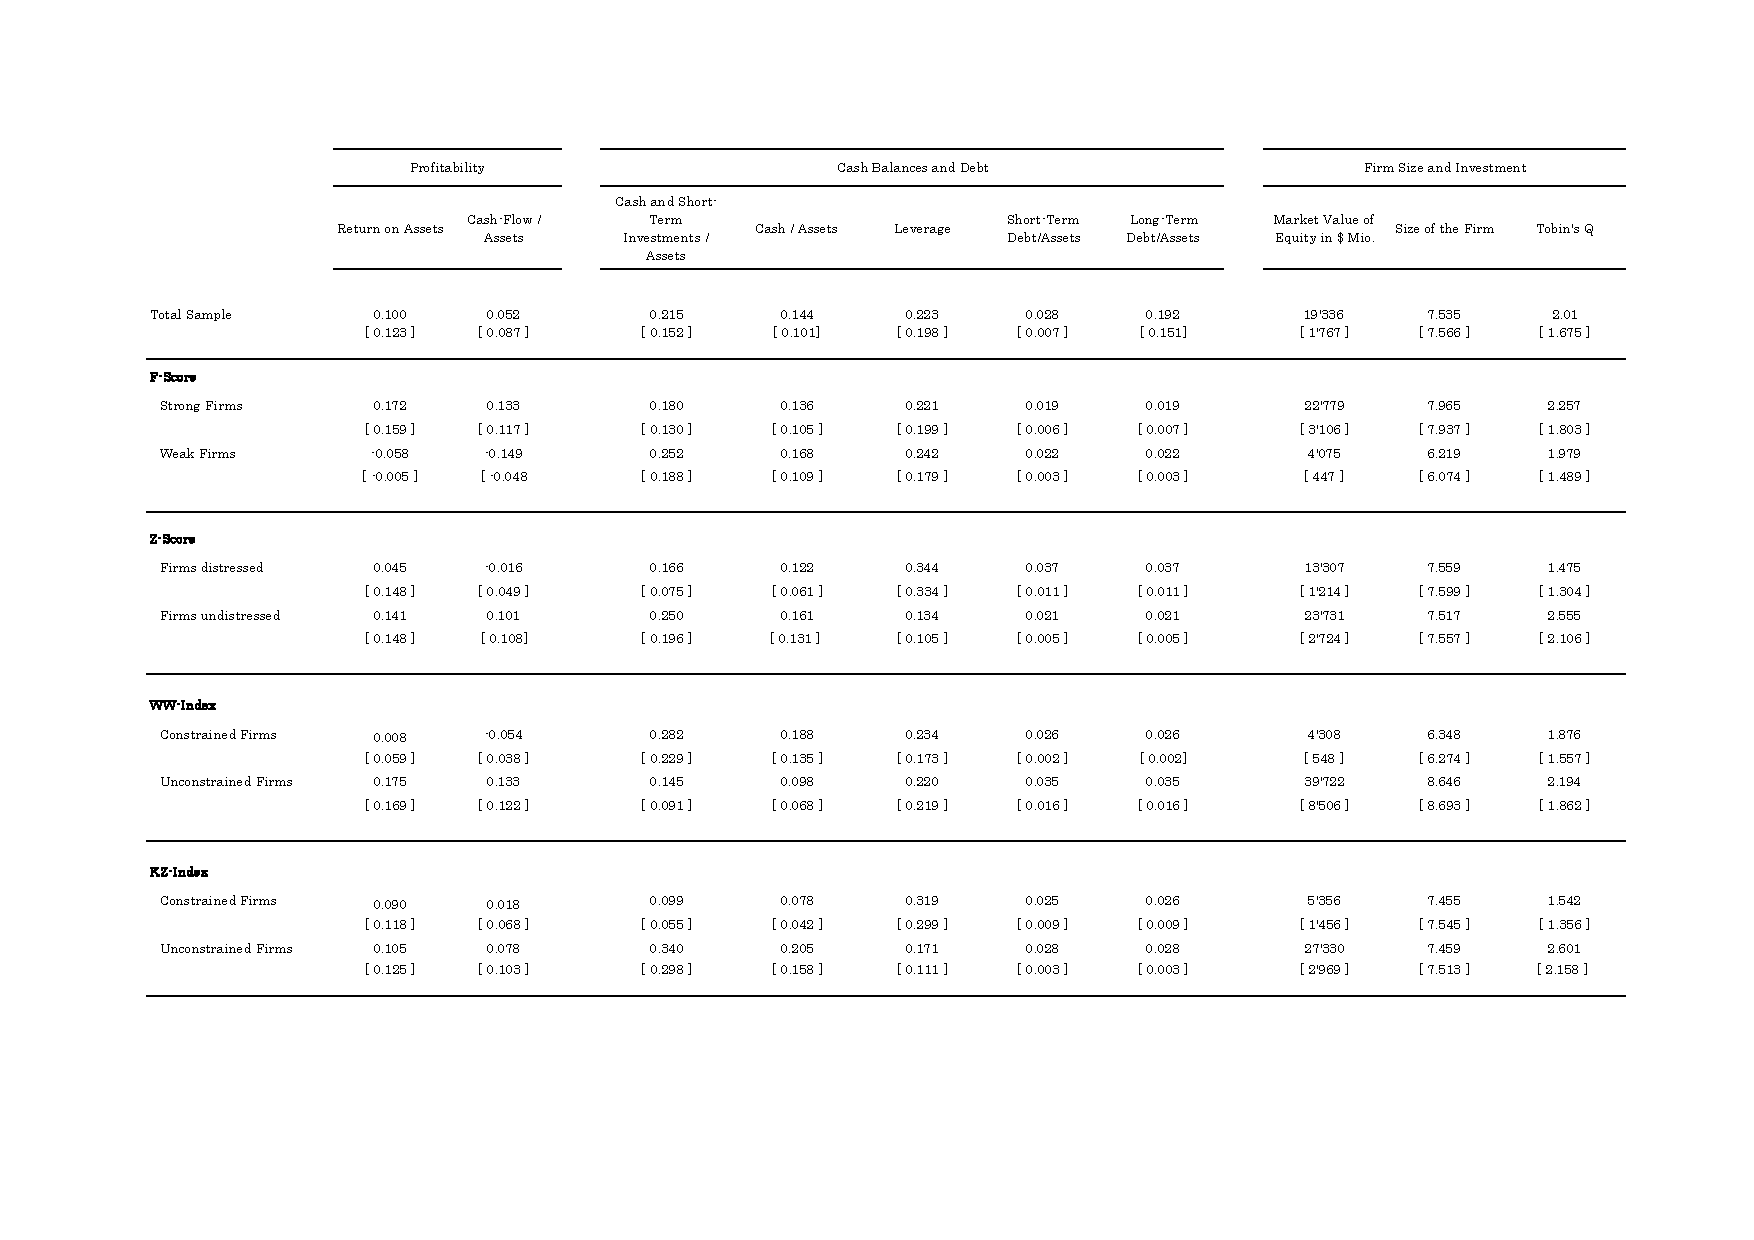
\includepdf[angle={90},pages={1},pagecommand={}, width=\textwidth]{Summary_by_Measurement_copy.pdf}
Panel B shows fundamentals on cash balances and debt in the form of cash and short-term investments, cash, short-term debt and long term debt, each divided by total assets and the variable leverage. According to \citep{MacKay2005} leverage is defined as the ratio of total debt to total assets. 
In Panel B, the ratio of cash and short-term investments and cash to assets have an uneven distribution across the samples. Weak and Whited-Wu constrained firms have higher ratios for both when compared to their counter samples. For the variable leverage however, samples of firms in a weaker financial condition have higher leverage compared to their counter sample. This is in line with the general understanding.
Panel C presents information on firm size and investment. The associated variables are market value of equity, the size of the firm defined as the natural logarithm of total assets and Tobin's Q. Tobin's Q and size are of importance as Tobin's Q is a proxy for investment opportunity \citep[p.957]{DUCHIN2010} and the size of firms in comparison can be seen as a sign of strength. 
Interestingly, the sub-samples of investors in a good condition have a market value of equity at least US\$ 10 billion higher when compared to their counter samples. Interestingly, the size of the firm does seem to be rather consistent across all the samples which implies that size is independent of the strength measures. When compared to the distribution for the variable leverage, Tobin's Q is higher for all investors in a good condition.
Taken together, the findings suggest that, when compared to each other, the four different measures of a firm's financial condition separate the sample in a common way. Weak firms have a bad profitability, distressed and Whited-Wu constrained firms have a negative operational cash flow and all firms in the weak condition sample have significant lower Tobin's Q when compared to firms in a good state. 

\section{Market Returns to Initial 13(D) Filings -- Abnormal Stock Returns}
% Intention
Abnormal share price reactions around the filing date identify the effect the 13(D) filing has on the target's stock, after accounting for general market movements.
The set up of the event study performed for this purpose is as follows: The time line consists successively of the estimation window, in which parameter estimates are obtained, the event window for which the abnormal returns are computed and the post event window. 
The filing date, as reported by the SEC and reported on EDGAR is set as the event day. For simplicity, the event window [x,y] is determined relative to the event day 0 with x days before and y days after the filing date. Abnormal returns are computed for various event windows. For that reason, the estimation window is set 120 days prior to the largest event window. With the largest event window starting 30 days before the event day, the estimation window begins 150 days prior to the actual event day.\\
The abnormal return $AR_{i,t}$ for the target's security $i$ at day $t$ is defined as the difference between the actual (observed) return $R_{i,t}$ and the expected return $E(R_{i,t}|X{t})$ given the absence of the event \citep[p.15]{MacKinlay1997}:
	\begin{equation}\label{eq:1}
		AR_{i,t}=R_{i,t}-E(R_{i,t}|X_{t})
	\end{equation}
The expected return $E(R_{i,t}|X{t})$ is the result of an estimation based the market model, in which the value-weighted NYSE/Amex/Nasdaq index from CRSP proxies for the market return $R_{M,t}$ and likewise is the independent variable.
	\footnote{For the expected return the market model assumes a constant and linear relation between the observed returns $R_{i,t}$ and the return of a market index $R_{m,t}$ \citep[p.18]{MacKinlay1997}. The parameters are estimated by ordinary least squares regressions based on estimation-window observations of stock returns.}
This yields the abnormal return $AR_{i,t}$
	\begin{equation}\label{eq:2}
		AR_{i,t}=R_{i,t}-(\hat{\alpha_{i}}+\hat{\beta_{i}}R_{M,t})
	\end{equation}
To accommodate for a multiple period event window and to draw overall inferences of the Schedule 13(D) filings \citep[p.21]{MacKinlay1997}, the abnormal returns $AR_{i,t}$ for target $i$ are aggregated over the event window $(\tau_1,\tau_2)$. 

For robustness, two different methods in aggregating over time are used. The cumulative abnormal return $CAR_{i,(\tau_1,\tau_2)}$ and the abnormal buy-and-hold return $BHAR_{i,(\tau_1,\tau_2)}$.\\
The cumulative abnormal return $CAR_{i,(\tau_1,\tau_2)}$ for security $i$ in event window $(\tau_1,\tau_2)$, is the sum of the abnormal returns $AR_{i,t}$ from equation \eqref{eq:2}.
	\begin{equation}
		CAR_{i,(\tau_1,\tau_2)}=\sum_{t=1}^{T}AR_{i,t}
	\end{equation}
\pagebreak

The second method of aggregation over time is the abnormal buy-and-hold return $BHAR_{i,(\tau_1,\tau_2)}$. It is independent from the results of equation \eqref{eq:2} and no estimation window is required. 
The abnormal buy-and-hold returns $BHAR_{i,(\tau_1,\tau_2)}$ are the difference between the realized (observed) buy-and-hold returns and the normal buy-and-hold returns $R(R_{i,t}|X_{t})$.
But in contrast to the cumulative abnormal return, the buy-and-hold return mimics the investment strategy of investors that buy the stock and hold it for a longer period of time. In this sense, the actual (normal) buy-and-hold return on day $t$ is the return on day $t$ times its lagged return on day $t_{-1}$. This means that for the target's security $i$ in the event window $(\tau_1,\tau_2)$ the abnormal buy-and-hold return $BHAR_{i,(\tau_1,\tau_2)}$ is
\begin{equation}
	BHAR_{i,(\tau_1,\tau_2)}=\prod_{t=1}^{T}(1+R_{i,t})-\prod_{t=1}^{T}(E(R_{i,t}|X_{t})
\end{equation}
Analogous to the estimation of normal returns for equation \eqref{eq:2}, the value-weighted NYSE/Amex/Nasdaq index from CRSP is used to calculate the normal buy-and-hold returns in the respective event windows $(\tau_1,\tau_2)$.

\subsection{Univariate I}

Graph 1 plots the mean CAR and BHAR over the event window [-30,30]. A first glance reveals that both methods generate almost similar results. Around 5 days prior to the filing date, the mean buy-and-hold return increases in magnitude and continues to proceed above the average cumulative abnormal return.\\
Alarming is the fact that in either case, the market processes almost all information before the filing is actually announced. The first impact on the securities prices occurs at around day -7 so information -- in any form -- is available, before the filing is public. 
Section 13(d) specifies that after passing the 5\% threshold, a firm has a maximum of 10 days to file the Schedule 13(D). So in the window [-10,0] other public announcements corresponding with the investment can be made. If for example a takeover announcement is made public during the ten days in which the firm is not obligated to file, the abnormal returns might be due to the takeover announcement. This means, the filing itself has little impact and is just a necessary accompaniment.  With regards to the remaining purposes of transaction, there is no reason to believe they follow a similar pattern. 

\begin{figure}
	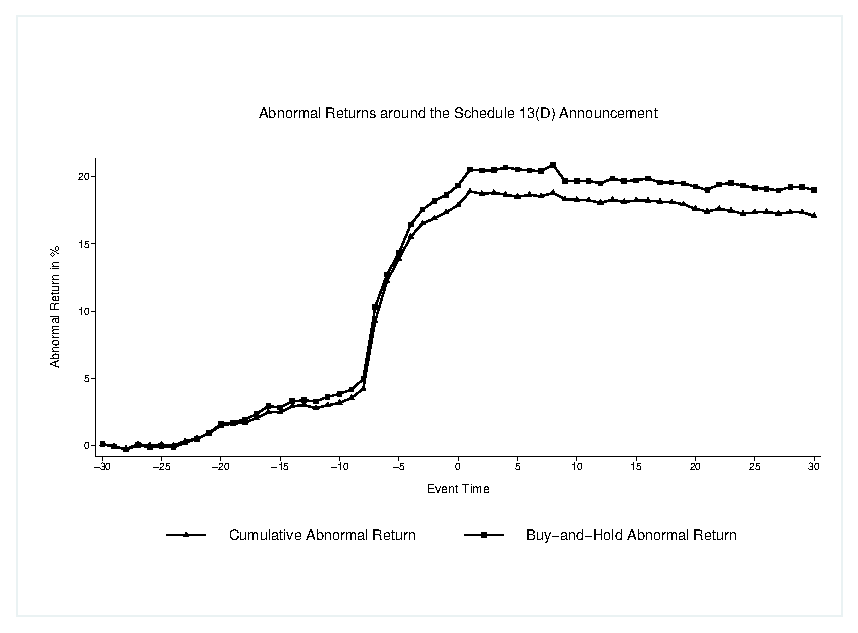
\includegraphics{Abnormal_Returns.eps} \label{AR both}
\end{figure} 

A scenario in which a different announcement triggers the abnormal share price reaction is conceivable. So when assessing the true impact of the filing, all abnormal returns in the event-window [-10,0] should be neglected and only those occurring after the announcement, including the event day, should be utilized. This however is a limited approach, as the announcement still affects the abnormal returns in the event window of the filing and a strict separation over time would not mitigate all the announcement effects. \\
To put this scenario into perspective, \citet[p.32]{Brigida2012} observe that most informed trading on 13(D) filings is conducted during the event-window [-10,-6] and that the runup is the greatest during this period. This is perfectly matching with the abnormal returns presented in Graph I. Additionally, filings can be processed overnight and are published only the next day so enlarging the event window to at least [-1,x] seems to be a sensitive measure. An even larger event window is applied by \citet[207]{Klein2009} beginning at day -30 to allow for the 10-day 13(D) filing window and possible prior leakage of information. They however, analyse the investment behavior of hedge funds and other private investors. \\
In an attempt to isolate possible effects of takeover announcements on abnormal returns around day -7, a second graph excluding takeover filings was plotted. The graph showed that abnormal returns primarily decrease in magnitude and that the early impact on the target's stock remained at around day -7. This means that even when controlling for the largest sub-sample which simultaneously is the only one for which an earlier announcement is plausible, the early impact is still existing. 

For the above mentioned reason, table III shows aggregated abnormal returns for the following five event windows: Event window 1 is [-10,3] to allow for the 10-day filing window and accommodate subsequent press coverage. The second event window is [-10,-6] to isolate the possible effect of earlier announcements on the target's stock around day -7. Analogous the third event window is [-5,3] to allow for information leakages but control for other announcements. The fourth event window is [-1,3] to accommodate the above scenario but relax the assumption of no inclusion of abnormal returns that occur before the filing day. 

Panel A-D show the mean [median] cumulative and buy-and-hold abnormal returns for each of the four event windows. Column (1) presents the abnormal returns for the complete sample. In a first attempt to detect differences in abnormal returns for firms with investors in different financial conditions, Column (2) and (3) show the abnormal returns for the filing sub-samples of strong and weak investors. They are equal to the sub-samples presented in Table II and grouped based on their F-score. Column (4) tests the difference in means [medians] of column (2) and (3). All returns presented in Table III are winsorized at the 1\% and 99\% level.

Panel A presents the abnormal returns for the largest event window [-10+3], neglecting the possibility that the abnormal returns are also driven by other announcements. Both CAR and BHAR are positive and strongly significant at the 1\% level with abnormal returns . Targets that belong to the sub-sample of filings submitted by strong investors have a mean CAR and BHAR 2.5\% higher when compared to weak investors. The difference in medians is around 7\% and strongly significant. 

In panel B similar results can be seen. For the complete sample the mean CAR and BHAR have almost the same size with 9.24\% and 9.30\% and are statistically significant at the 1\% level. Strong firms again have higher abnormal returns but the difference is not statistically significant. 

The event window [-5,3] in Panel C tries isolate a possible strong effect of prior announcements on the abnormal returns. Although it does not completely isolate a possible announcement effect (the event window of a filing would overlap with the post event window of such an announcement) it is set to work as an approximation. When compared to the following event window [-5,3] in Panel C, the mean abnormal returns of Panel B are larger although it only includes the abnormal returns of five days compared to nine days. It is in particular interesting, as more than half of the abnormal returns in the event window [-10,3] occur in the days [-10,-6]. 

Panel D presents the abnormal returns for the shortest and tightest event window around the filing date [-1,3]. Both measures show positive significant abnormal returns. However, for the complete sample is the median close to zero which suggests that the aggregated abnormal returns are distributed with a left skew. 

Concluding, abnormal returns on stocks subject to Schedule 13(D)'s filed by corporations experience a significant positive market reaction around the filing date. Apparent is the economic difference in abnormal returns for stocks belonging to either filings submitted by strong or weak investors. Across all event windows does the abnormal return of targets with a strong investor outperform those of weak investors. Even in the event-window [-1,3] is the economic difference more than 20\% in relative terms with Panel A and C showing statistically significant differences in the medians of the sub-samples. 

\pagebreak

\subsection{Abnormal Stock Returns by Purpose of Initial 13(D) Filing}


  

\begin{comment}
	
\section{Indentifying the Financial Condition of the Investor}
% Objective -- What is the financial condition? 
% Topics: Composition | Elements | Procedure
 

\subsection{Piotroskis F-Score -- A Measurement of Financial Strength}
%Objective -- How do we characterized strong firms? 
%Topics: Descrription | Why | Outlook 

In a study of 2010, \emph{BCG} noted many of that year's acquisitions would involve a financially strong acquirer. However, the attribute of being financially strong is not ambivalent. Piotroski's F-Score adresses this issue as it is a "... composite measure of firm strength" \citep[p. 496]{Fama2006}. It consists of nine binary signals which consider in what directions the fundamentals of a company are trending and whether general health conditions are met \citep{Mohr2012}. \citet{Piotroski2000} established it to seperate strong from weak value firms
	\footnote{In order to legitimize the explanatory power of the F-score in separating strong from weak firms Piotroski formed portfolios consisting of value firms. In doing so, he showed that an investment strategy of shorting expected losers (weak firms) and buying expected winners (strong firms) would "generate a 23\% average annual return" \citep[p. 4]{Piotroski2000}. This is matching with \citet{Hyde2014} results, who observe significant return premiums for stocks with a high F-score over stocks with a low F-score.}
. 
Although the F-score was established to distinguish among value firms, \citet{Mohr2012} shows that its application on growth stocks yields similar results.
	\footnote{This is in line with \citet{Piotroski2000} and confirms earlier research conducted by him.}. 
With regards to the above, the F-Score is used to divide the complete sample of investors into strong and weak ones.

\subsection{The Whited-Wu Index -- A Measurement of Financial Constraints}
A firm is financially constrained if it faces an inelastic supply of external capital \citep{Farre-mensa2013} and those who are able to raise substential amounts of external capital without much of an increase in the cost of capital are unconstrained. Although \citet{Khatami2014} notes that more recent literature has questioned the reliability of constraint measures, the Whited-Wu Index as in \citet{Liao2010} is used as an indicator. 


\subsection{Altman's Z-Score -- A Measurement of Financial Distress}
Financial distress describes a state in which a company cannot meet or has difficulty paying off, its financial obligatiosn to its creditors. In this sense, HNA Group could be in a state of financial distress as they have problems refinancing the debt burden, and recently planned to sell their stake in Hilton Worldwide Holdings Inc. to pay down a large pile of debt. Altman's Z-score is a widely accepted measure of financial distress. The fundamental indicator shows statistically significant results in predicting the bankruptcy of a company \citep{Campbell2008} and is still applied as a general practical tool for assessing the financial well-being of firms \citep{Kleinert2014}. 
	\footnote{The model consists of five financial ratios that are coefficients by discriminate analysis method where the financial ratios are independent variables of it. The five financial ratios of the Z-score are (1) working capital to total assets, (2) retained earning to total assets, (3) earnings before interest and taxes to total assets, (4) market value of equity to book value total debt and (5) sales to total assets. This yields
		\begin{equation}
			Z=1.2(X_{1})+1.4(X_{2})+3.3(X_{3})+0.6(X_{4})+0.999(X_{5})
		\end{equation}
	The cut-off point is at Z=2.675 where a lower score implies bankruptcy of a firm and a higher score non-bankruptcy.}
.

\subsection{Other Measurements}

\subsection{Tobin's Q}
Tobin's Q is included because it proxies for a firm's investment opportunity which assesses the 
\footnote{In accordance with \citet{Brigida2012}, Tobin's Q is defined as 
\begin{equation}
	Tobin's Q= \frac{MVE + PSE + Debt}{AT}
\end{equation}, where $MVE$ is the market capitalization, $PSE$ is the lquidating value of preferred stock, $Debt$.. } 
\citep{DUCHIN2010}. According to \citet{Khatami2014} constrained firms have higher tobin's Q compared to unconstrained firms, which may be due to their unexploted investment opportunities \citep{Khatami2014}.

\subsection{Company Size}
Company size 



\pagebreak

It was established by Altman in his 1968 paper 


In conducting the analysis, the F-score will be used to separate  the sample of 13D filings among strong and weak corporate investors. Since is is able to separate firms in portfolios into strong and weak performing ones, an application to this analysis seems reasonable. 
%insert negative aspects here - accruals 
However, components of the f-score include changes in leverage and The score itself can be divided into the three dimensions profitability, balance sheet health and operating efficiency. 
In the context of this analysis As \citet{Mohr2012} states: the f-score considers in what direction the fundamentals of a company are trending and whether financial health conditions are met.  Because high F-scores imply higher returns hence stronger firms should have higher returns, investors must see a high F-score as a representation of financial strength. In the context of this paper those practices would have only been applied to the target and not the investor. An application of the F-score on the investor with the aim of distinguishing between strong and weak firms 


\citet{Choi2012} formulate it from a target perspective - "does financial strength predict subsequent institutional demand"? 

%In general, analyzed characteristics across the sample of filings but not the characteristics of the parties in general.

On the other hand, \citet{Akhigbe2007} examine the characteristics of final acquisitions following partial bids. They find that involvements by corporate bidders are more likely to result in a full acquisition. 

% previous studies have examined the content of the filings and therefre indirectly involved the investor in their analysis and when actively involving a party only analysed the target (s. above paragraph).
% difference of the paper 
\end{comment}

\section{Appendix}

\subsection{Appendix A}
In order to compute the abnormal returns $AR_{i,t}$ for security $i$ at time $t$ in \eqref{eq:1} the following models are used: 
\begin{enumerate}
	\item Market Model -- For the expected return it assumes a constant and linear relation between the observed returns $R_{i\tau}$ and the return of a market index $R_{m\tau}$. The parameters are estimated by ordinary least squares regressions based on estimation-window observations. The value-weighted NYSE/Amex/Nasdaq index from CRSP is used as the market return $R_{M\tau}$.

		\begin{equation}
			R_{i,\tau}=\alpha_{i}+\beta_{i}R_{M,\tau}+\epsilon_{i,\tau}
		\end{equation}
		with 
		\begin{equation}
			E[\epsilon_{i,\tau}]=0
		\end{equation}
		and 
		\begin{equation}
			Var[\epsilon_{i,\tau}]=\sigma^2_{i,\tau}
		\end{equation}
		This yields the abnormal return $AR_{i,\tau}$
		\begin{equation}
			AR_{i,\tau}=R_{i,\tau}-(\hat{\alpha_{i}}+\hat{\beta_{i}}R_{M,\tau})
		\end{equation}
		
	\item Market Return Model -- The model is classified as the restricted market model with $\alpha_{i}=0$ and $\beta_{i}=1$. This means that there is no estimation window required and the abnormal return $AR_{i,\tau}$ is simply the difference between the observed return $R_{i,\tau}$ and the value-weighted NYSE/Amex/Nasdaq index return $R_{M\tau}$.

		\begin{equation}\label{eq:6}
			AR_{i,\tau}=R_{i,\tau}-R_{M,\tau}
		\end{equation}

\end{enumerate}

\end{document}